\documentclass[a4paper,11pt,dvipdfmx]{jsarticle}


% 数式
\usepackage{amsmath,amsfonts}
\usepackage{bm}

% 画像
\usepackage[dvipdfmx]{graphicx}

% 図形
\usepackage{tikz}
\usetikzlibrary{shapes.geometric}
\usetikzlibrary {shapes.misc}

% ソースコード
\usepackage{listings,jlisting,color}
\lstset{
basicstyle={\ttfamily},
identifierstyle={\small},
commentstyle={\smallitshape},
keywordstyle={\small\bfseries},
ndkeywordstyle={\small},
stringstyle={\small\ttfamily},
frame={tb},
breaklines=true,
columns=[l]{fullflexible},
numbers=left,
xrightmargin=0zw,
xleftmargin=3zw,
numberstyle={\scriptsize},
stepnumber=1,
numbersep=1zw,
lineskip=-0.5ex
}
\renewcommand{\lstlistingname}{ソースコード}


\begin{document}

\title{インテリジェントシステム レポート課題1}
\author{21T2166D 渡辺大樹}
\date{\today}
\maketitle
\section{A*探索アルゴリズムでの探索}
\subsection{(a)AradからBucharestまで}
\subsubsection{A1 $f_1(n)=g(n)+D(n)$を用いた探索}
$f_1(n)=g(n)+D(n)$の評価関数を用いて探索を行った結果、Bucharestのノード情報は[12, Bucharest, 418, 418, 10]となった。

見つかった経路はArad→Sibin→Rimnicu Vilces→Pitesti→Bucharestとなった。

ゴールが見つかった時点でのfrontierはF値の順に[12, Bucharest, 418, 418, 10],

\noindent
[13, Craiova, 455, 615, 10],[14, Rimnicu Vilces, 514, 707, 10]となった。

せっかくなので以下に実際に展開されたSearch Treeを示す。

\newpage
\begin{tikzpicture}[
        level 1/.style={sibling distance=35mm, level distance=30mm},
        level 2/.style={sibling distance=35mm, level distance=35mm},
        level 3/.style={sibling distance=35mm, level distance=30mm},
        level 4/.style={sibling distance=35mm, level distance=30mm},
        every node/.style={text centered, text width=1.5cm, font=\small},
        TreeNode/.style={circle, draw}
    ]
    \node[TreeNode, blue] {Arad}
    child {
            node[TreeNode, teal] {Sibiu}
            child {node[TreeNode] {Arad}}
            child {node[TreeNode] {Fagaras}}
            child {node[TreeNode] {Oradea}}
            child {
                    node[TreeNode, teal] {Rimnicu Vilces}
                    child {node[TreeNode] {Craiova}}
                    child {
                            node[TreeNode, teal] {Pitesti}
                            child {node[TreeNode, red] {Bucharest}}
                            child {node[TreeNode] {Craiova}}
                            child {node[TreeNode] {Rimnicu Vilces}}
                        }
                    child {node[TreeNode] {Sibiu}}
                }
        }
    child {node[TreeNode] {Timisoara}}
    child {node[TreeNode] {Zerind}};

\end{tikzpicture}

\subsubsection{A2 $f_1(n)=g(n)+2 \cdot D(n)$を用いた探索}
$f_1(n)=g(n)+2 \cdot D(n)$の評価関数を用いて探索を行った結果、Bucharestのノード情報は[9, Bucharest, 460, 460, 6]となった。

見つかった経路はArad→Sibin→Fagaras→Bucharestとなった。

ゴールが見つかった時点でのfrontierはF値の順に[9, Bucharest, 460, 460, 6],

\noindent
[10, Sibiu, 338, 844, 6]となった。

こちらもせっかくなので以下に実際に展開されたSearch Treeを示す。
\newpage
\begin{tikzpicture}[
        level 1/.style={sibling distance=35mm, level distance=30mm},
        level 2/.style={sibling distance=35mm, level distance=35mm},
        level 3/.style={sibling distance=35mm, level distance=30mm},
        every node/.style={text centered, text width=1.5cm, font=\small},
        TreeNode/.style={circle, draw}
    ]
    \node[TreeNode, blue] {Arad}
    child {
            node[TreeNode, teal] {Sibiu}
            child {node[TreeNode] {Arad}}
            child {
                    node[TreeNode, teal] {Fagaras}
                    child {node[TreeNode, red] {Bucharest}}
                    child {node[TreeNode] {Sibiu}}
                }
            child {node[TreeNode] {Oradea}}
            child {node[TreeNode] {Rimnicu Vilces}}
        }
    child {node[TreeNode] {Timisoara}}
    child {node[TreeNode] {Zerind}};

\end{tikzpicture}

\subsection{(b)LugojからBucharestまで}
\subsubsection{A1 $f_1(n)=g(n)+D(n)$を用いた探索}
$f_1(n)=g(n)+D(n)$の評価関数を用いて、LugojからBucharestまでの探索を行った結果、この探索は失敗となった。
評価関数の値により、Lugoj→Mehadin→Lugoj→$\cdots$と冗長な経路となり、抜け出せなくなった。

以下が実際に展開されたSearch Treeとそのときの$\rm{F_1,G}$となる。

\begin{center}
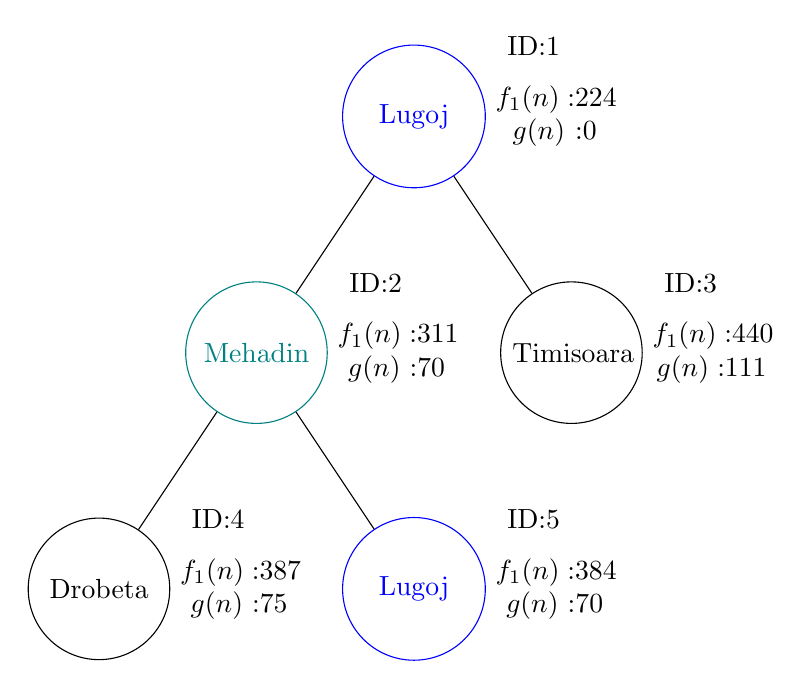
\begin{tikzpicture}[
        level 1/.style={sibling distance=40mm, level distance=30mm},
        level 2/.style={sibling distance=40mm, level distance=30mm},
        every node/.style={text centered, text width=1.5cm},
        TreeNode/.style={circle, x radius = 3cm, y radius = 2cm, rotate=0, draw}
    ]
    \node[TreeNode, blue](a) {Lugoj}
    child {
        node[TreeNode, teal](b) {Mehadin}
        child {node[TreeNode](d) {Drobeta}}
        child {node[TreeNode, blue](e) {Lugoj}}
    }
    child {node[TreeNode](c) {Timisoara}};

    \node also [label=right:$f_1(n):$224\\$g(n):$0] (a);
    \node also [label=above right:ID:1] (a);

    \node also [label=above right:ID:2] (b);
    \node also [label=right:$f_1(n):$311\\$g(n):$70] (b);

    \node also [label=above right:ID:3] (c);
    \node also [label=right:$f_1(n):$440\\$g(n):$111] (c);

    \node also [label=above right:ID:4] (d);
    \node also [label=right:$f_1(n):$387\\$g(n):$75] (d);

    \node also [label=above right:ID:5] (e);
    \node also [label=right:$f_1(n):$384\\$g(n):$70] (e);

\end{tikzpicture}
\end{center}

\subsubsection{A2 $f_1(n)=g(n)+2 \cdot D(n)$を用いた探索}
$f_1(n)=g(n)+2 \cdot D(n)$の評価関数を用いて、LugojからBucharestまでの探索を行った結果、A1と同じくこの探索は失敗となった。
評価関数の値により、Lugoj→Mehadin→Lugoj→$\cdots$と冗長な経路となり、抜け出せなくなった。

以下が実際に展開されたSearch Treeとそのときの$\rm{F_1,G}$となる。

\begin{center}
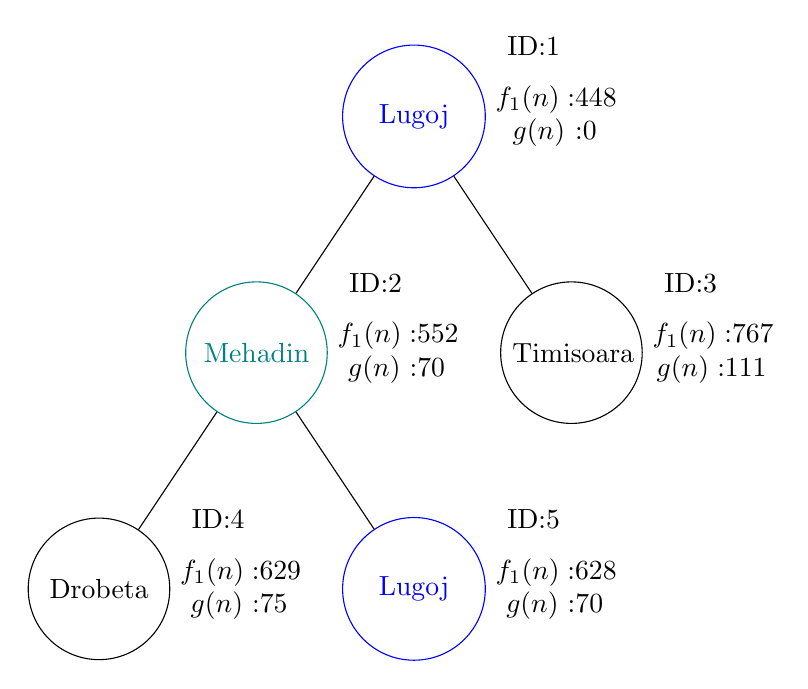
\begin{tikzpicture}[
        level 1/.style={sibling distance=40mm, level distance=30mm},
        level 2/.style={sibling distance=40mm, level distance=30mm},
        every node/.style={text centered, text width=1.5cm},
        TreeNode/.style={circle, x radius = 3cm, y radius = 2cm, rotate=0, draw}
    ]
    \node[TreeNode, blue](a) {Lugoj}
    child {
        node[TreeNode, teal](b) {Mehadin}
        child {node[TreeNode](d) {Drobeta}}
        child {node[TreeNode, blue](e) {Lugoj}}
    }
    child {node[TreeNode](c) {Timisoara}};

    \node also [label=right:$f_1(n):$448\\$g(n):$0] (a);
    \node also [label=above right:ID:1] (a);

    \node also [label=above right:ID:2] (b);
    \node also [label=right:$f_1(n):$552\\$g(n):$70] (b);

    \node also [label=above right:ID:3] (c);
    \node also [label=right:$f_1(n):$767\\$g(n):$111] (c);

    \node also [label=above right:ID:4] (d);
    \node also [label=right:$f_1(n):$629\\$g(n):$75] (d);

    \node also [label=above right:ID:5] (e);
    \node also [label=right:$f_1(n):$628\\$g(n):$70] (e);

\end{tikzpicture}
\end{center}

\section{ヒューリスティック関数の許容性について}
この課題では以下の$h_a \sim h_f$が許容的であるかを調べる。

許容的とは、すべてのノードに対してヒューリスティック関数が示す予想最小コスト$h(n)$が
そのノードからの実際の最小コストとなる$h^*(n)$以下になることをいう。

すなわち以下に与えられる関数$h_a \sim h_f$に対し、すべてのnで$h_x(n) \leq h^*(n)$を言えればその関数は許容的であるといえる。

ただし、$1 \leq i \leq k$の$i$について$h_i(n) \leq h^*(n)$(すなわち許容的)である。
\subsection{$h_a(n)$}
$h_a(n)$は
\begin{equation*}
    h_a(n) = \sum_{i=1}^{k}h_i(n)
\end{equation*}
の関数となる。

この関数$h_a(n)$が$h^*(n)$以下になるとき、許容的であるといえる。
ここで$h_i(n) \leq h^*(n)$より$h_1(n), h_2(n) = h^*(n)$であるとすると少なくとも$h_a(n)$は
\begin{equation*}
    h_a(n) \geq 2 \cdot h^*(n)
\end{equation*}
であるといえる。

したがって$h_a(n)$は許容的ではない。

\subsection{$h_b(n),h_c(n)$}
$h_b(n)$は
\begin{equation*}
    h_b(n) = \max\{h_1(n),h_2(n),h_3(n),\cdots,h_k(n)\}
\end{equation*}
の関数となる。

この関数$h_b(n)$が$h^*(n)$以下になるとき、許容的であるといえる。
$\max$関数は$h_1(n),h_2(n),h_3(n),\cdots,h_k(n)$の関数の中から最大となる関数を選ぶ関数である。
$h_i(n) \leq h^*(n)$より任意の$h_i(n)$において許容的となるため、$\max$関数によってどの関数が選ばれても$h_b(n)$は許容的である。

$h_c(n)$も同様であり、$h_c(n)$は
\begin{equation*}
    h_c(n) = \min\{h_1(n),h_2(n),h_3(n),\cdots,h_k(n)\}
\end{equation*}
の関数となる。

上記にあるようにこちらも$\min$関数の働きを考えれば$h_c(n)$は許容的であるといえる。

\subsection{$h_d(n)$}
$h_d(n)$は
\begin{equation*}
    h_d(n) = \prod_{i=1}^{k}h_i(n)
\end{equation*}
の関数となる。

この関数$h_d(n)$が$h^*(n)$以下になるとき、許容的であるといえる。
ここで$h_i(n) \leq h^*(n)$より$h_1(n), h_2(n) = h^*(n)$であるとすると少なくとも$h_d(n)$は
\begin{equation*}
    h_d(n) \geq \{h^*(n)\}^2
\end{equation*}
であるといえる。

したがって$h_d(n)$は許容的ではない。

\subsection{$h_e(n)$}
$h_e(n)$は
\begin{equation*}
    h_e(n) = \frac{1}{k}\sum_{i=1}^{k}h_i(n)
\end{equation*}
の関数となる。

この関数$h_e(n)$が$h^*(n)$以下になるとき、許容的であるといえる。
ここで$h_i(n) \leq h^*(n)$より、$h_i(n)$をすべてが最大値である$h_1(n),h_2(n),h_3(n),\cdots,h_k(n) = h^*(n)$であるとするとその総和は
\begin{equation*}
    \sum_{i=1}^{k}h_i(n) = k \cdot h^*(n)
\end{equation*}
となる。ここで両辺を$k$で割れば
\begin{equation*}
    \frac{1}{k}\sum_{i=1}^{k}h_i(n) = h^*(n)
\end{equation*}
となる。したがって
\begin{equation*}
    h_e(n) = h^*(n)
\end{equation*}
と表せる。$h_1(n),h_2(n),h_3(n),\cdots,h_k(n) < h^*(n)$であれば
\begin{equation*}
    h_e(n) < h^*(n)
\end{equation*}
であるので、これを組み合わせることで
\begin{equation*}
    h_e(n) \leq h^*(n)
\end{equation*}
といえる。

したがって$h_e(n)$は許容的である。

\subsection{$h_f(n)$}
$h_f(n)$は
\begin{equation*}
    h_f(n) = \sum_{i=1}^{k}\omega_i h_i(n)
\end{equation*}
の関数となる。(ただし$0<\omega_i,\sum_{i=1}^{k}\omega_i = 1$)

この関数$h_f(n)$が$h^*(n)$以下になるとき、許容的であるといえる。
ここで$h_i(n) \leq h^*(n)$より、$h_i(n)$をすべてが最大値である$h_1(n),h_2(n),h_3(n),\cdots,h_k(n) = h^*(n)$であるとするとその総和は
\begin{equation*}
    \sum_{i=1}^{k}\omega_ih_i(n) = h^*(n) \cdot \sum_{i=1}^{k}\omega_i
\end{equation*}
となる。ここで$0<\omega_i,\sum_{i=1}^{k}\omega_i = 1$より
\begin{equation*}
    \sum_{i=1}^{k}\omega_ih_i(n) = h^*(n)
\end{equation*}
となる。したがって
\begin{equation*}
    h_f(n) = h^*(n)
\end{equation*}
と表せる。$h_1(n),h_2(n),h_3(n),\cdots,h_k(n) < h^*(n)$であれば
\begin{equation*}
    h_f(n) < h^*(n)
\end{equation*}
であるので、これを組み合わせることで
\begin{equation*}
    h_f(n) \leq h^*(n)
\end{equation*}
といえる。

したがって$h_f(n)$は許容的である。

\subsection{ヒューリスティック関数を用いた探索}
ここでは以下のヒューリスティック関数$\bar{h}$を用いてA*アルゴリズムを適応した時の結果について考える。
\subsubsection{(a):$\bar{h}(n)=\frac{1}{2}h(n)$}
$\bar{h}(n)=\frac{1}{2}h(n)$のとき、$h(n)$が許容的であることから
\begin{equation*}
    h(n) \leq h^*(n)
\end{equation*}
となる。この式の両辺を2で割れば
\begin{equation*}
    \frac{1}{2} h(n) \leq \frac{1}{2} h^*(n) < h^*(n)
\end{equation*}
と表すことができる。そのため$\bar{h}$は許容的であり、最適コストの経路が見つかる。

\subsubsection{(b):$\bar{h}(n)=\frac{4}{5}h(n) + \frac{1}{5}h^*(n)$}
$\bar{h}(n)=\frac{4}{5}h(n) + \frac{1}{5}h^*(n)$のとき、$h(n)$が許容的であることから
\begin{equation*}
    h(n) \leq h^*(n)
\end{equation*}
となる。この式の両辺に$\frac{4}{5}$をかければ
\begin{equation*}
    \frac{4}{5} h(n) \leq \frac{4}{5} h^*(n) 
\end{equation*}
と表すことができる。この式にさらに$\frac{1}{5}h^*(n)$を足すことで
\begin{equation*}
    \frac{4}{5} h(n) + \frac{1}{5}h^*(n) \leq h^*(n) 
\end{equation*}
とでき、与式の右辺が$h^*$よりも小さいことが確認できる。

このことから$\bar{h}$は許容的であり、最適コストの経路が見つかる。

\subsubsection{(c):$\bar{h}(n)=2h(n)$}
$\bar{h}(n)=2h(n)$のとき、$h(n)$が許容的であることから
\begin{equation*}
    h(n) \leq h^*(n)
\end{equation*}
となる。この式の両辺を2でかけると
\begin{equation*}
    2 h(n) \leq 2 h^*(n) 
\end{equation*}
と表すことができる。しかしこの式では$\bar{h}$が許容的であることは示せないため、この$\bar{h}$では最適コストの経路が見つからない。

\subsubsection{(d):(c)での経路コスト$C$}
経路コストはそれを$C$と置くと、ノードnまでのコストとノードnでのヒューリスティック関数をそれぞれ$g(n),h(n)$とすることで
\begin{equation*}
    C = g(n) + h(n) 
\end{equation*}
と表せる。

ここで全問(c)でのヒューリスティック関数が$\bar{h}(n)=2h(n)$より、
\begin{equation*}
    C = g(n) + 2h(n) 
\end{equation*}
となる。ここで$h(n)$が許容的であるためノードnからの最小コストを$h^*(n)$とすると
\begin{equation*}
    C \leq g(n) + 2h^*(n) 
\end{equation*}
上記(c)からわかるようにこのヒューリスティック関数では最小コストの経路が見つからない。

経路探索では$2h(n)$のヒューリスティック関数を用いているのでノードnまでの最適経路を$g^*(n)$とすれば
ノードnまでの経路コストは$g(n) \leq 2g^*(n)$となる。したがって式は
\begin{equation*}
    C \leq 2g^*(n) + 2h^*(n) 
\end{equation*}
となる。したがって最小コストを$C^*$とすれば
\begin{equation*}
    C \leq 2C^*
\end{equation*}
が得られる。

\end{document}